\documentclass[crop,tikz]{standalone}
\usetikzlibrary{positioning,arrows,fit,calc,shapes.symbols,shapes.geometric}
\pgfdeclarelayer{bg}
\pgfsetlayers{bg,main}
\tikzset{
	>=stealth'
}
\makeatletter
\pgfdeclareshape{document}{
	\inheritsavedanchors[from=rectangle] % this is nearly a rectangle
	\inheritanchorborder[from=rectangle]
	\inheritanchor[from=rectangle]{center}
	\inheritanchor[from=rectangle]{north}
	\inheritanchor[from=rectangle]{south}
	\inheritanchor[from=rectangle]{west}
	\inheritanchor[from=rectangle]{east}
	% ... and possibly more
	\backgroundpath{% this is new
		% store lower right in xa/ya and upper right in xb/yb
		\southwest \pgf@xa=\pgf@x \pgf@ya=\pgf@y
		\northeast \pgf@xb=\pgf@x \pgf@yb=\pgf@y
		% compute corner of ‘‘flipped page’’
		\pgf@xc=\pgf@xb \advance\pgf@xc by-7.5pt % this should be a parameter
		\pgf@yc=\pgf@yb \advance\pgf@yc by-7.5pt
		% construct main path
		\pgfpathmoveto{\pgfpoint{\pgf@xa}{\pgf@ya}}
		\pgfpathlineto{\pgfpoint{\pgf@xa}{\pgf@yb}}
		\pgfpathlineto{\pgfpoint{\pgf@xc}{\pgf@yb}}
		\pgfpathlineto{\pgfpoint{\pgf@xb}{\pgf@yc}}
		\pgfpathlineto{\pgfpoint{\pgf@xb}{\pgf@ya}}
		\pgfpathclose
		% add little corner
		\pgfpathmoveto{\pgfpoint{\pgf@xc}{\pgf@yb}}
		\pgfpathlineto{\pgfpoint{\pgf@xc}{\pgf@yc}}
		\pgfpathlineto{\pgfpoint{\pgf@xb}{\pgf@yc}}
		\pgfpathlineto{\pgfpoint{\pgf@xc}{\pgf@yc}}
	}
}
\makeatother

\begin{document}
	
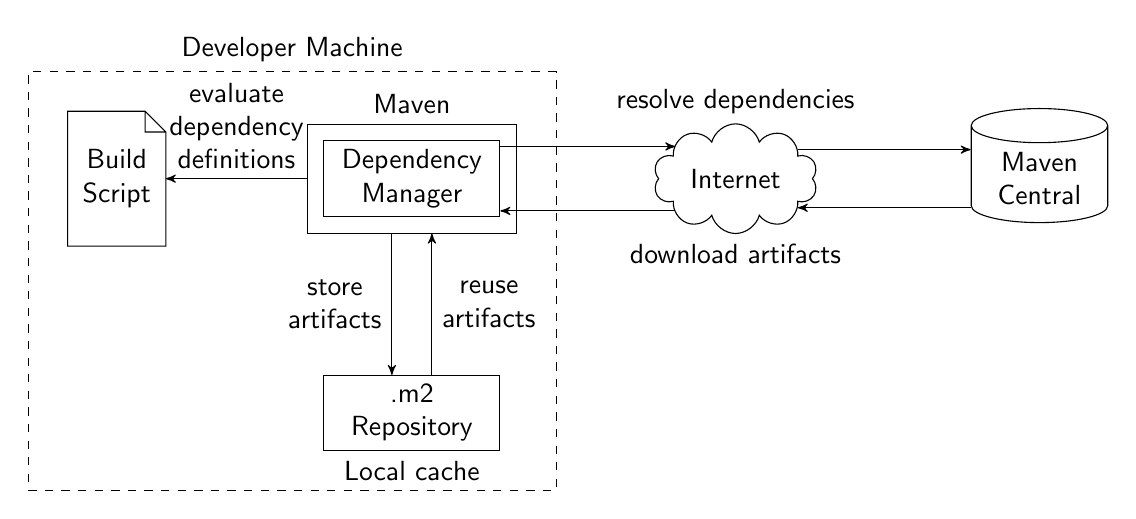
\begin{tikzpicture}[
node distance = 20mm,
every node/.style = {
	font = \sffamily
},
script/.style = {
	shape=document,
	draw,
	%line width=1pt,
	text width=1cm,
	minimum height=1.7cm,
	align=center
},
component/.style = {
	draw,
	%line width=1pt,
	text width = 2cm,
	align = center	
},
internet/.style = {
	draw,
	cloud,
	aspect=2	
},
database/.style = {
	draw,
	cylinder,
	shape border rotate=90,
	aspect=0.25,
	text width = 1.5cm,
	align = center
}
]
	
\node[script] (script) {Build Script};
	
\node[component, right=of script] (depMgr) {Dependency Manager};

\node[draw, fit=(depMgr), inner sep=2mm] (maven) {};
\node[above=0mm of maven] {Maven};

\node[component, below=of depMgr] (local) {.m2\\ Repository};
\node[below=0mm of local] {Local cache};

\node[draw, dashed, fit={(maven)(local)(script)}, inner sep = 5mm] (pc) {};
\node[above=0mm of pc] {Developer Machine};

\node[internet, right=of depMgr] (internet) {Internet};
\node[above=0mm of internet] {resolve dependencies};
\node[below=0mm of internet] {download artifacts};

\node[database, right=of internet] (central) {Maven Central};

\draw[->] (maven) -- node[above, text width=2cm, align=center] {evaluate dependency definitions} (script);	

\draw[->] (maven.250) -- node[left, text width = 2cm, align=center, xshift=4mm] {store artifacts} (maven.250 |- local.north);
\draw[->] (maven.290 |- local.north) -- node[right, text width = 2cm, align=center, xshift=-4mm] {reuse artifacts} (maven.290);

\draw[->] (depMgr.20) -- +(22.2mm,0);
\coordinate[right=22.2mm of depMgr.340] (dmgrr);
\draw[->] (dmgrr) -- +(-22.2mm,0);

\draw[->] (internet.25) -- (internet.25 -| central.west);
\draw[->] (internet.335 -| central.west) -- (internet.335);
	
\end{tikzpicture}

\end{document}